%!TEX root = main.tex


\section{Causal Bayesian Networks}\label{sec:CBN}

\todo[inline]{Vague variable = observable variable. The connotations of the latter make explanations a bit more intuitive. Also, somehow explain ``latent variables are things we use to make models''}

What is a causal Bayesian network? We will consider a simplified case where a single node may be intervened on. With this condition, according to \citet{pearl_causality:_2009}, a causal Bayesian network is a probability model $\prob{P}$, a collection of interventional probability models $\{\prob{P}_{\RV{X}=a}|a\in X_i\}$ and a directed acyclic graph $\mathcal{G}$ whose nodes are identified with some collection of variables, which we can group into three variables $\{\RV{W},\RV{X},\RV{Y}\}$, where $\RV{W}$ is the sequence of variables associated with the parents of $\RV{X}$ in $\mathcal{G}$, $\RV{X}$ is the ``intervenable'' node of $\mathcal{G}$ and $\RV{Y}$ are associated with the other nodes. The interventional probability models must all obey the truncated factorisation condition with respect to $\mathcal{G}$:
\begin{align}
    \prob{P}_{\RV{X}=a}^{\RV{W}\RV{X}\RV{Y}}(w,x,y) &= \prob{P}^{\RV{W}}(w)\prob{P}^{\RV{Y}|\RV{XW}}(y|x,w)\llbracket x=a \rrbracket\label{eq:truncated_fac2}
\end{align}

\todo[inline]{Prove this is equivalent to the normal definition}

What are these variables $\{\RV{W},\RV{X},\RV{Y}\}$, and what do we mean they are distributed according to $\prob{P}$? To begin with, it means that observations are modeled by a sequence of variables $\RV{V}_A:=(\RV{W}_i,\RV{X}_i,\RV{Y}_i)_{i\in A}$, for which we assume the triples $(\RV{W}_i,\RV{X}_i,\RV{Y}_i)$ are mutually independent and identically distributed but we are not sure exactly how they are distributed. This can be captured by introducing a latent variable $\RV{H}$representing the distribution of $\RV{V}_i:=(\RV{W}_i,\RV{X}_i,\RV{Y}_i)$ for any $i\in A$\footnote{Under the theory introduced we are implicitly assuming $\RV{H}$ to be finite. It would clearly be desirable to extend the theory so that we can weaken this assumption, but it doesn't prevent us from explaining the basic idea.}. Then we define a model of observations such that $\model{T}^{\RV{V}_i|\RV{H}}=\model{T}^{\RV{V}_j|\RV{H}}$ (for any $i,j\in A$) and $\RV{V}_i\CI_{\model{T}}\RV{V}_j|\RV{H}$. Then, the assumption ``given a probability model $\prob{P}$'' can be identified with the definition 
\begin{align}
    \prob{P}:=\model{T}^{\RV{V}_i|\RV{H}}(\cdot|h)\text{ for some }h\in H\text{ and any }i\in A\label{eq:what_is_p}
\end{align}

What do the interventional probability models represent? We have already established on the basis of observations that the variables $\RV{W},\RV{X},\RV{Y}$ don't represent ``observables'' in the sense we discuss in Section \ref{sec:variables} -- we cannot explain which observation specifically $\RV{W}$ represents. We will suppose, as with observations, that there is some set $B$ such that $\RV{V}_B$ are a sequence of observables modeled by the interventional models but we will leave $B$ unspecified for now. 

We also know that interventional probability models are coupled to observational models via $\RV{H}$. That is Equations \ref{eq:truncated_fac2} and \ref{eq:what_is_p} together indicate that for different values $h,h'\in H$, we will generally get different sets of interventional models. We can define a collection of models of interventions $\model{U}^{\RV{V}_B|\RV{H}}_{\RV{X}_B=a}$ such that $\RV{V}_i$ are independent and identically distributed conditional on $\RV{H}$ and for any $i\in B$, $j\in A$:
\begin{align}
    \model{U}^{\RV{W}_i\RV{X}_i\RV{Y}_i|\RV{H}}_{\RV{X}_i=a}(w,x,y|h) &= \model{T}^{\RV{W}_j|\RV{H}}(w)\model{T}^{\RV{Y}_j|\RV{X_jW_jH}}(y|x,w,h)\llbracket x=a \rrbracket \label{eq:truncated_fac3}
\end{align}
This is just the same as Equation \ref{eq:truncated_fac2}, except we make the coupling between $\model{T}$ and $\model{U}$ via $\RV{H}$ explicit. We will also modify the notation in one more way. Instead of considering a collection of interventional models, we'll consider the map $\kernel{U}:=a\mapsto \model{U}^{\RV{V}_B|\RV{H}}_{\RV{X}_B=a}$. $\kernel{U}$ is a Markov kernel, and to make it a model we need to specify the domain and codomain indices. It can inherit the codomain index $(\RV{V}_B)$ from the original interventional interventional models, and its domain index is clearly going to be $(\RV{H},RV{Q})$ for some $\RV{Q}$ -- i.e. it will also inherit $\RV{H}$ in its domain index. 

To work out what the remaining variable $\RV{Q}$ ought to be, the question we need to answer is: when we supply a value $a$ to $\kernel{U}$, \emph{which observable variable are we saying takes the value $a$}?  Consider that we refer to interventions by invoking the variable $\RV{X}_i$, as in the subscript ``$\RV{X}_i=a$'' (or, in alternative notation, $do(\RV{X}_i=a)$). Furthermore, Equations \ref{eq:truncated_fac2} and \ref{eq:truncated_fac3} force $\RV{X}$ to be deterministically equal to the argument of $\RV{U}$. For these reasons (and others we will see below), we think it is reasonable to choose $\RV{X}_B$ to be the remaining domain index of $\model{U}$. Thus we have:
\begin{align}
    \model{U}^{\RV{V}_B|\RV{HX}_B}(v|h,a) &= \model{U}^{\RV{V}_B|\RV{H}}_{\RV{X}_B=a}(v|h)\\
    \model{U}^{\RV{W}_i\RV{X}_i\RV{Y}_i|\RV{HX}_i}(w,x,y|h,a)&=\model{U}^{\RV{W}_i\RV{X}_i\RV{Y}_i|\RV{H}}_{\RV{X}_i=a}(w,x,y|h)
\end{align}
And we stipulate that $(\RV{W}_i\RV{X}_i\RV{Y}_i)\CI_\model{U} \RV{V}_{B\setminus \{i\}} | \RV{H}\RV{X}_i$, which is makes the second line well-defined (without this we would have to condition on $\RV{X}_B$).

We intentionally left the sets $A$ and $B$ vague. Let's consider the possibility that they overlap; that is, there is some $i\in A\cap B$. We can express the coupling between observational and interventional models by joining them with a copymap, as follows:
\begin{align}
    \tikzfig{cbn_seedo}\label{eq:inconsistent_cbn}
\end{align}

However, \ref{eq:inconsistent_cbn} cannot usually be a model. Because the variable $\RV{V}_i$ appears twice, unless we force the output at each terminal to be deterministically equal, which limits us to modelling deterministic functions of $\RV{H}$, then this model is inconsistent (see Lemma \ref{lem:nocopy1}). Thus we can conclude that, usually, $B\cap A=\emptyset$, that is to say observations are typically distinct from consequences. 

\emph{Purely to avoid introducing new graphical notation}, we will suppose that $A=\{1\}$ and $B=\{2\}$. Because the sequences are conditionally independent and identically distributed, we can construct a model of arbitrary length sequences $A$ and $B$ from length-one examples. However, we will leave this construction implicit.

If we assume that the triples are $(\RV{W}_i,\RV{X}_i,\RV{Y}_i)$ are mutually variationally independent for all $i\in A\cup B$, then we can also extend $\model{T}$ as follows:
\begin{align}
    \model{T}^{\RV{V}_{A\cup B}|\RV{HX}_{B}} &:= \tikzfig{cbn_sd2}\\
    \model{U}^{\RV{W}_i\RV{X}_i\RV{Y}_i|\RV{HX}_i} &= \tikzfig{truncated_fac_definition}\\
    \implies \model{T}^{\RV{V}_{A\cup B}|\RV{HX}_{B}} &= \tikzfig{cbn_sd23}\label{eq:cbn_maybe_comb}
\end{align}

So we have in Equation \ref{eq:cbn_maybe_comb} a definition of a model $\model{T}$ which, we argue, is the general form of a model of observables implied by the original definition of a causal Bayesian network (recall that our definition restricted interventions to target a single node). The model in Equation \ref{eq:cbn_maybe_comb} looks like a 2-comb:
\begin{align}
    \tikzfig{cbn_sd_2comb} \label{eq:cbn_2comb}
\end{align}

To actually \emph{be} a 2-comb we require a family of ``inserts'' $\model{S}^{\RV{X}_B|\RV{V}_A\RV{W}_B}$ that, in combination with $\model{T}^{\RV{V}_{A\cup B}|\RV{HX}_{B}}$,  generate models $\model{P}^{\RV{V}_{A\cup B}|\RV{H}}$. However, after this surprisingly long journey, a hypothesis presents itself to us: perhaps $\model{T}^{\RV{V}_{A\cup B}|\RV{HX}_{B}}$ is a see-do model, and the appropriate family of inserts are strategies.

There is only one problem with this. If $\model{T}^{\RV{V}_{A\cup B}|\RV{HX}_{B}}$ is a see-do model, then $\RV{X}_B$ is the variable representing decisions. However, the range of $\RV{X}_j$, $j\in B$ is exactly the same as the range of $\RV{X}_i$, $i\in A$. In general, there's no reason to expect that the observations we make will have the same range as the decisions available. To return to our favourite example, we might have observations $\RV{X}$ of body mass index, but the decision $\RV{D}$ we are considering might be whether or not to go on a diet. A more generic see-do model might then be of the form $\model{T}^{\RV{V}_{A\cup B}|\RV{HD}}$ for some decision variable $\RV{D}$.

Given a generic $\model{T}^{\RV{V}_{A\cup B}|\RV{HD}}$, there exists a conditional probability $\model{T}^{\RV{V}_{A\cup B}|\RV{HX}_{B}}$ if and only if $\RV{V}_{A\cup B}\CI_{\model{T}} \RV{D}|(\RV{H,X}_B)$. This implies that there exists some $\RV{T}^{\RV{X}_B|\RV{W}_B\RV{HD}}$ such that
\todo[inline]{Prove it!}
\begin{align}
    \model{T}^{\RV{V}_{A\cup B}|\RV{HD}} &= \tikzfig{cbn_sd_2comb_extended}
\end{align}



In the presentation of \citet{pearl_causality:_2009}, a Causal Bayesian Network posits an observational probability distribution such as $P(X,Y)$, and a set of interventional distributions, for example $\{\prob{P}_h(X,Y|do(X=x))\}_{x\in X,h\in H}$. Here we use notation similar to typical notation used for Causal Bayesian Networks and don't intend for these to necessarily be elements of any modelling context. For simplicity, we will consider a Causal Bayesian Network with only hard interventions on a single variable, e.g. interventions only of the form $do(\RV{X}=x)$.

First we will offer some commentary



We can consider this an instance of a see-do model. To do so consistently within a modelling context $\mathscr{M}$, we need to distinguish observation and intervention variables - let the former retain the labels $\RV{X},\RV{Y}$ and call the latter $\RV{X}',\RV{Y}'$. Let $D=\{do(\RV{X}=x)\}_{x\in X}$. Then a Causal Bayesian Network can be considered a see-do model $\model{T}[\RV{XYX'Y'}|\RV{HD}]$ by identifying $\model{T}[\RV{XY}|\RV{H}]_h := \prob{P}_h(X,Y)$ and $\model{T}[\RV{X'Y'}|\RV{HD}]_{h,do(\RV{X}=x)}:={P}_h(X,Y|do(X=x))$.

\todo[inline]{We need to rename the consequence variables because otherwise we would have $\model{T}[\RV{XYXY}|\RV{HD}]$ and the two $\RV{X}$'s and the two $\RV{Y}$'s would be deterministically equal by the ``identical labels'' rule}

We can say a bit more about Causal Bayesian Networks. Suppose we have the network
\begin{align*}
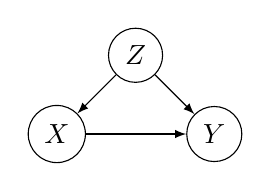
\begin{tikzpicture}
    \path (0,0) node[draw,circle] (X) {$\RV{X}$}
    ++ (1,1) node[draw,circle] (Z) {$\RV{Z}$}
    ++ (1,-1) node[draw, circle] (Y) {$\RV{Y}$};
    \draw[-latex] (X)--(Y);
    \draw[-latex] (Z) -- (Y);
    \draw[-latex] (Z) -- (X);
\end{tikzpicture}
\end{align*}

Then, letting $\model{T}[\RV{XYZ}|\RV{H}]$ be the observational ``see'' model and $\model{T}[\RV{X'Y'Z'}|\RV{HD}]$ be the interventional ``do'' model with $D$ the set of interventions $\{do(\RV{X}=x)\}_{x\in X}$ where we write $x:=do(\RV{X}=x)$ for short, then we know by the backdoor adjustment rule that $\model{T}[\RV{X'Y'Z'}|\RV{HD}]_{hx}^{x'yz} \overset{krn}{=} \model{T}[\RV{Z}|\RV{H}]_h^z \delta[x]^{x'} \model{T}[\RV{Y}|\RV{XZH}]_{hx'z}^y$. 

Let $\model{U}[\RV{ZY}|\RV{XH}] = \model{T}[\RV{Z}|\RV{H}]\rightrightarrows \model{T}[\RV{Y}|\RV{XZH}]$, call $\model{T}[\RV{X}|\RV{H}]$ the ``observational strategy'' and $\model{D}_x[\RV{X}|\RV{D}]_x^{x'} \overset{krn}{=} \delta[x]^{x'}$ the interventional strategies for all $x\in X$. Then we have

\begin{align}
    \model{T}[\RV{XYZ}|\RV{H}] &= \model{U}[\RV{Z}|\RV{H}]\rightrightarrows \model{T}[\RV{X}|\RV{H}] \rightrightarrows \model{U}[\RV{Y}|\RV{XHZ}]\\
    \model{T}[\RV{X'Y'Z'}|\RV{HD}] &\overset{krn}{=} \model{U}[\RV{Z}|\RV{H}]\rightrightarrows \model{D}[\RV{X}|\RV{D}] \rightrightarrows \model{U}[\RV{Y}|\RV{XHZ}]
\end{align}
So this simple example of a Causal Bayesian network is a ``nested comb'' where the outer comb $\model{T}[\RV{XYZX'Y'Z'}|\RV{HD}]$ is the ``see'' and ``do'' models, which are themselves generated by the inner comb $\model{U}[\RV{ZY}|\RV{XH}]$ with different choices $ \model{T}[\RV{X}|\RV{H}]$ and $\model{D}[\RV{X}|\RV{D}]$ for the insert.

This is a simple example, but \citet{jacobs_causal_2019} has used an ``inner comb'' representation of a general class of Causal Bayesian Networks to prove a sufficient identification condition which is itself slightly more general than the identification condition given by \citet{tian2002general}.